\cotefile{80}
\scanpage{55}
Soient $a,b,c$ les sommets de $K_J$, $\alpha,\beta,\gamma$
les sommets ``opposés'' dans $K_{J'}=K_I$, intersections
de $D_a$ avec la ps. dr. joignant $b$ \unsure{:|à} $c$ etc ;
\unsure{soit|soient} $\lambda_a,\lambda_b,\lambda_c$ les arêtes de $K_I$ \unsure{contenant|conten$^{\mathrm{t}}$}
$\alpha,\beta,\gamma$, alors $\{\lambda_a,\lambda_b,\lambda_c\}$ est comp. avec
l'orientation.

En résumé

\uline{Théorème} Le foncteur canonique
du groupoïde des arrang$^{\mathrm{mts}}$ de
\unsure{ps.droites|pseudodroites} sans bigone, vers \inserted{celui} des arrangements
1 dimensionnels de pseudo-droites (sans
bigone) est pleinement fidèle.

Les conditions $(A1)$ à $(A6)$ donnent
en principe une voie pour déterminer
l'image essentielle -- mais il faut \unsure{d'|et|dt}
doit arriver à simplifier les conditions
en question. En principe, il faudrait
encore rajouter la relation d'EP (23) --
mais je soupçonne que cette dernière
est automatique.
% archive sheet number: 54

\scanpage{57}
\figure{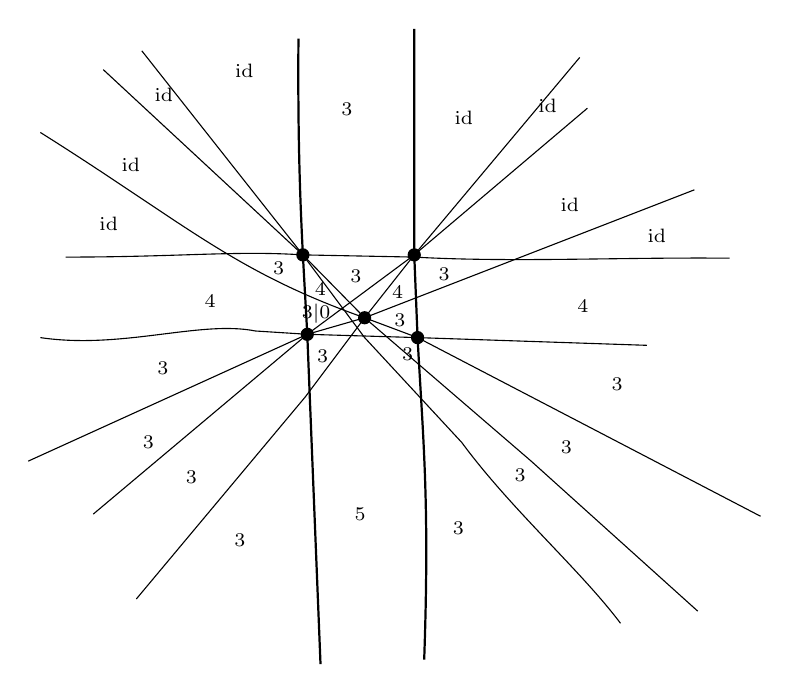
\begin{tikzpicture}[x=.014cm,y=-.014cm,every node/.style={inner sep=0pt,font=\scriptsize}]
\draw[thick] (269,31) .. controls (268,160) and (273,224) .. (277,299) -- (289,598);
\draw[thick] (374,22) -- (374,227) -- (377,302) .. controls (382,395) and (388,450) .. (383,594);
\draw (58,229) .. controls (161,229) and (212,223) .. (273,227) -- (374,229) .. controls (462,234) and (562,229) .. (660,230);
\draw (35,302) .. controls (109,313) and (180,286) .. (230,296) -- (277,299) -- (377,302) -- (585,309);
\draw (35,116) .. controls (167,199) and (210,242) .. (329,284) -- (377,302) -- (688,464);
\draw (92,59) -- (273,227) -- (329,284) -- (480,414) -- (631,550);
\draw (127,42) -- (273,227) -- (329,302) -- (417,397) .. controls (462,458) and (524,512) .. (561,561);
\draw (24,414) -- (277,299) -- (329,284) -- (628,168);
\draw (83,462) -- (277,299) -- (374,227) -- (531,94);
\draw (122,539) -- (275,356) -- (329,284) -- (374,227) -- (524,48);
\foreach \x/\y in {273/227,277/299,329/284,374/227,377/302} \fill (\x,\y) circle[radius=6];
\foreach \x/\y in {220/60,147/82,117/145,97/199,419/103,495/92,515/182,594/210} \node at (\x,\y) {id};
\foreach \x/\y in {313/95,251/239,321/246,401/245,361/286,291/319,368/317,146/330,133/397,172/429,216/486,414/475,470/427,512/401,558/344} \node at (\x,\y) {$3$};
\node at (285,280) {$\unsure{3|0}$};
\foreach \x/\y in {189/269,289/258,359/261,527/274} \node at (\x,\y) {$4$};
\node at (325,462) {$5$};
\end{tikzpicture}}
\margin{$\left(\begin{array}{l}+\,9\ \text{triangles}\\+\,1\ \text{carré}\end{array}\right)$}

\margin{25 triangles\\5 carrés\\1 pentagone}

\margin{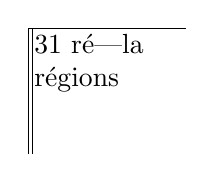
\begin{tikzpicture}[baseline=(r.base)]\node[anchor=north west,align=left,inner sep=2pt](r) at (0,0) {31 \deleted{\unsure{ré|la}}\\régions};\draw (0,-1.6)--(0,0)--(2,0);\draw (.05,-1.6)--(.05,0);\end{tikzpicture}}
% archive sheet number: 56

\scanpage{58}
\figure{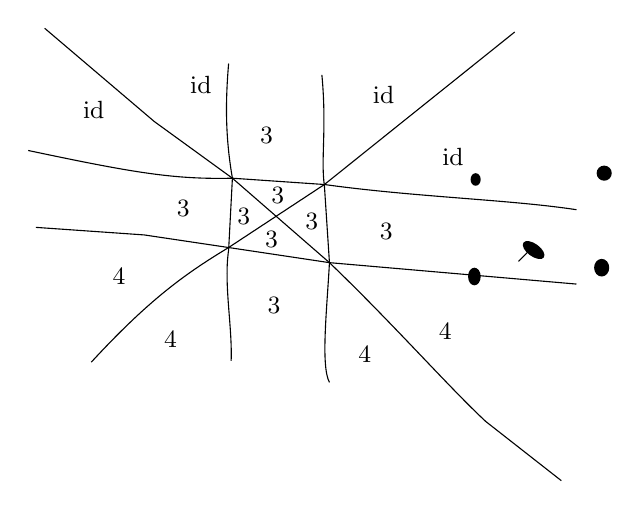
\begin{tikzpicture}[x=.016cm,y=-.016cm,every node/.style={font=\small,inner sep=0pt}]
\draw (291,137) .. controls (288,172) and (289,199) .. (294,228) -- (291,285) .. controls (287,312) and (294,345) .. (293,373);
\draw (365,146) .. controls (369,189) and (364,213) .. (367,234) -- (371,295) .. controls (369,332) and (364,377) .. (371,390);
\draw (132,206) .. controls (217,224) and (248,229) .. (294,228) -- (367,233) .. controls (439,243) and (515,245) .. (567,253);
\draw (138,267) -- (224,273) -- (291,283) -- (371,295) -- (567,312);
\draw (145,109) -- (232,183) -- (294,228) -- (371,295) .. controls (422,344) and (465,393) .. (495,421) -- (555,468);
\draw (182,374) .. controls (229,323) and (258,303) .. (291,283) -- (367,233) -- (518,112);
\foreach \x/\y in {184/174,269/154,414/162,469/211} \node at (\x,\y) {id};
\foreach \x/\y in {321/194,255/252,303/258,330/242,357/262,325/277,416/270,327/329} \node at (\x,\y) {$3$};
\foreach \x/\y in {204/306,245/356,399/368,463/350} \node at (\x,\y) {$4$};
\fill (487,229) ellipse [x radius=4,y radius=5];
\fill (589,224) ellipse [x radius=6,y radius=6];
\fill (486,306) ellipse [x radius=5,y radius=7];
\fill[rotate around={-36:(533,285)}] (533,285) ellipse [x radius=10,y radius=5];
\draw (521,294) -- (530,285);
\fill (587,299) ellipse [x radius=6,y radius=7];
\end{tikzpicture}}
% archive sheet number: 57

\scanpage{59}
\figure{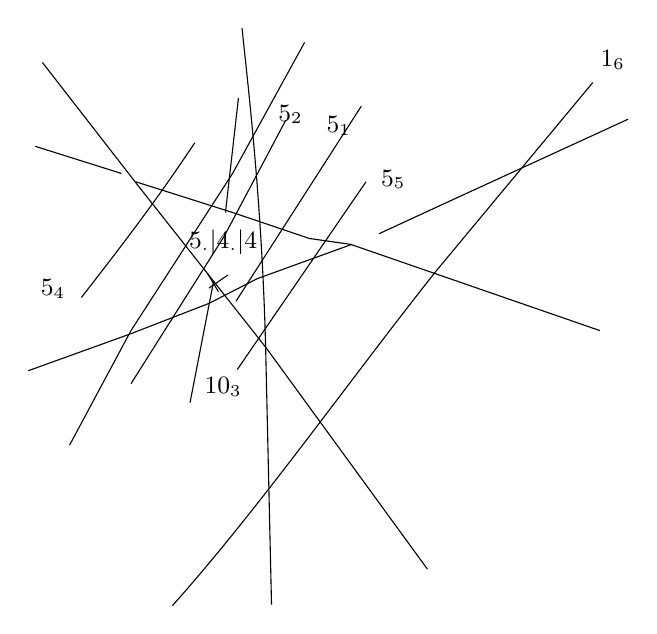
\begin{tikzpicture}[x=.015cm,y=-.015cm,every node/.style={font=\small,inner sep=0pt}]
\draw (148,67) -- (228,170) -- (337,308) -- (474,496);
\draw (142,138) -- (215,161); \draw (227,168) -- (309,194) -- (374,216) -- (409,221) -- (620,294);
\draw (136,328) -- (222,297) -- (289,271) -- (330,250) -- (410,221); \draw (433,212) -- (498,182) -- (644,115);
\draw (181,266) .. controls (216,221) and (243,186) .. (277,135);
\draw (171,391) -- (223,294) -- (309,161) -- (370,50);
\draw (223,339) -- (302,214) -- (354,116);
\draw (273,355) -- (293,252); \draw (303,194) -- (314,97);
\draw (312,269) -- (418,104); \draw (313,327) -- (422,168);
\draw (317,38) .. controls (324,103) and (334,193) .. (337,308) -- (342,526);
\draw (258,527) .. controls (332,444) and (405,340) .. (481,244) -- (614,84);
\node at (157,259) {$5_4$}; \node at (358,111) {$5_2$};
\node at (399,121) {$5_1$}; \node at (445,166) {$5_5$};
\node at (301,219) {$\unsure{5_{.}|4_{.}|4}$};
\draw (288,246) -- (297,261); \draw (289,258) -- (305,247);
\node at (301,342) {$10_3$}; \node at (631,65) {$1_6$};
\end{tikzpicture}}
\[
\begin{array}{rl}
5 &\\
15 &=5+10\\
10 &=5+5\\
1 &\\ \cline{1-1}
31 &
\end{array}
\]
\[
\begin{aligned}
1_6&\equiv\text{icosaèdre}\\
5_1&\equiv\text{hexagone}\\
5_4,5_2&\equiv\text{triangle bordé}\\
5_5,10_3&\equiv\text{carré gammé}
\end{aligned}
\]
% archive sheet number: 58

\scanpage{61}
\uline{Système de Pseudodroites}

\uline{Définition} : c'est une carte (topologique ou combinatoire)
dont la surface sousjacente $X$ est un plan projectif\textsuperscript{*}
% margin note written sideways
\margin{* i.e. (compacte) non orientable et de car. EP égale à 1\ldots}
réel, dont les ordres des sommets sont pairs $\geq4$ (d'où
la division de l'ensemble des arêtes en classes
d'équivalence, appelées les ``pseudodroites'' de la
carte) telles que deux pseudodroites se rencontrent
en un point et un seul.

\uline{Premières conséquences} : le nb \inserted{\deleted{\unsure{$p$}} $n$} des pseudodroites est $\geq2$.
L'immersion de $\mathbb{S}^1$ \unsure{ds|de|dans} $\mathbb{P}_{\mathbb{R}}^2$ correspondant à une
ps. dr. est (des deux classes d'isotopie possibles) celle
qui est non homotope à \deleted{\unsure{un}} $0$, i.e. le long d'une
psdr. $X$ est non orientable, i.e. la situation est la
\unsure{m\textsuperscript{e}|$=$} que pour une \uline{droite} (projective) dans le plan
projectif. On montre que pour des psdr ``en
position générale'' (sommets tous d'ordre 4) et
en nb $n\leq6$, la situation peut être \unsure{réalisé|réalisée} par
un système de vraies droites dans le plan
projectif réel.

Soit $D$ une pseudodroite de $X$, $\widetilde X$ le revêtement des
orientations de $X$ ($\widetilde X\simeq\mathbb{S}^2\simeq\mathbb{P}_{\mathbb{C}}^1$), $\widetilde D$ l'image inverse
de $D$ dans $X$. Alors $\widetilde X\setminus\widetilde D$ a deux comp.
connexes (ou ``hémisphères'') en corr. 1-1 can.
avec l'ens. des deux orientations de $D$.

Notons que \inserted{sur} l'ens. des sommets se trouvant
% archive sheet number: 60

\scanpage{62}
sur une même $D$ il y a une structure
polygonale induite (cela a un sens \inserted{clair} si
le nb $s_D$ de ces sommets est $\geq3$). \inserted{L'ens.} des
orientations de $D$ (ou encore, l'ens. $\pi_0(\widetilde X\setminus\widetilde D)$)
est en corr. 1-1 avec l'ens. des orientations
\deleted{\unsure{de la}} de ce polygône combinatoire. \deleted{(Si $s_D=2$ ou $s_D=1$}
% slanted
\margin{Il vaut peut être mieux dire que $D$ est le support d'un 1-sous-complexe du squelette $K^1$ de dim 1 de la carte et ce sous-complexe est un polygône comb. d'ordre $s_D$ (sans exclure les cas $s_D=1$ ou $s_D=2$\ldots)}

Soit $s$ un sommet de la carte. Si on exclut le
cas où toutes les psdr. sont ``concourrantes'' en $s$
(auquel cas $s$ est l'unique sommet), il
existe donc une $D$ qui ne passe pas par $s$,
et l'ens \inserted{$\Omega_s(\unsure{x|X})$} des orientations de $X$ en $s$ est en
corr 1-1 can. avec l'ens \inserted{$\Omega(D)$} des orientations
du polygône comb. $D$ (qui est défini en
termes du 1-complexe $K^1$ et de sa décomposition en psdroites\ldots) Mais soit $D'$ \deleted{\unsure{et $D''$}}
une autre psdroite ne passant pas par $s$, comment
expliciter la bijection composée
\diagram{\begin{tikzcd}[ampersand replacement=\&,column sep=small,row sep=small]
\Omega(D)\arrow[rr,dash,"\sim"]\arrow[dr,"\sim"'] \& \& \Omega(D')\\
\& \Omega_s(x)\arrow[ur,"\sim"] \&
\end{tikzcd}}
? \deleted{Si par $s$} Comme $s$ est d'ordre $\geq4$,
il passe par $s$ deux psdroites $\Delta,\Delta'$, \deleted{\unsure{soient}} \inserted{supposons}
qu'on puisse \deleted{\unsure{les}} choisir $\Delta$ \uline{et} $\Delta'$ non \unsure{concourrantes|concourantes} avec $D,D'$, soient
$u,u'$ (resp. $v,v'$) les int. de $\Delta$ (resp. $\Delta'$) avec $D,D'$,
dont l'int est désignée par $t$. On constate alors
(puisque la configuration des quatre psdroites
% archive sheet number: 61

\scanpage{63}
$D,D',\Delta,\Delta'$ est en position générale, donc en
position \unsure{standard|standart}) que $\overrightarrow{tu\unsure{v|u}}$ et $\overrightarrow{tu'v'}$ se correspondent.
[Plus généralement, si on a $k$ droites
$\Delta_1\ldots\Delta_k$ passant par $s$ et non par $t$, \inserted{et coupant $D$ en $u_i$ et $D'$ en $u'_i$,} et si
on prend sur $D\setminus\{t\}$ et $D'\setminus\{t'\}$ les relations
d'ordre \inserted{induites par des orientations de $D,D'$} qui se correspondent, alors si on ordonne
les $\Delta_i$ de façon que les \deleted{$D$} $u_i$ aillent en
croissant, de \unsure{m\textsuperscript{e}|$=$} les $u'_i$.] Ceci explicite la
bijection $\Omega(D)\simeq\Omega(D')$ en termes de la
combinatoire du $K^1$ et de ses ps-droites
sauf dans le cas où il n'y a qu'une seule ps-droite \inserted{$\Delta$} passant par $s$ et non par $t$, (ce qui implique
qu'il existe \unsure{exact$^{\mathrm{mt}}$|exactement} 2 psdr passant par $s$, i.e. que
l'ordre de $s$ est 4 \unsure{\}|)}, et qu'il existe une ps.dr. $\Delta'$
passant par $s$ et par $t$) Supposons qu'il existe une
ps.dr. $D''$ \inserted{ne passant pas par $t$} distincte des \unsure{$\Delta'$ en|$\Delta'$} (i.e. que la figure
% slanted
\margin{NB $D''$ ne passe pas par $s$ i.e. cette ps.dr. $\ne\Delta,\Delta'$}
ne se réduise à un faisceau des ps.dr. passant
par $t$, et une sécante $\Delta$ de ce faisceau) --
elle \deleted{est} \deleted{\unsure{passe}} \deleted{\unsure{donc}} $\ne\Delta,\Delta',D,D'$ et ne passe pas par $s$
Soient $x,x'$ les pts d'int. de $D''$ avec $D,D'$ et $u,u'$
ceux de $\Delta$ avec $D,D'$. Si on a $x\ne u$, $x'\ne u'$, alors
on peut comparer par ce qui précède les \deleted{\unsure{orientations}} \inserted{ensembles}
% archive sheet number: 62

\scanpage{64}
\deleted{\unsure{de}} $\Omega(D'')$ \deleted{\unsure{et}} et $\Omega(D)$, et $\Omega(D'')$ et $\Omega(D')$, donc
$\Omega(D)$ et $\Omega(D')$, et on gagne. Si par contre
\unsure{toutes|t\textsuperscript{tes}} les psdroites qui ne passent pas par $t$ passent
par $u$, ou si elles passent toutes par $u'$, on est
dans le cas des deux faisceaux de ps. droites,
de sommet $t$ et $u$ (resp. $u'$), qui demande
encore un traitement à part. Mais supposons
qu'il n'existe pas de $D''$ qui ne passe ni par
$u$ ni par $u'$ (ni par $t$, bien-entendu) mais
qu'il en existe \inserted{$\unsure{\Gamma|\Gamma_1}$} qui ne passe pas par $u'$, \inserted{(mais par $u$)} et d'autres qui ne passe par $u^{\deleted{\unsure{\prime}}}$ (mais par $u'$), alors
\figure{\begin{tikzpicture}[x=.013cm,y=-.013cm,every node/.style={font=\scriptsize,inner sep=1pt}]
\draw (68,339) -- (208,272) -- (467,151) -- (596,105);
\draw (59,309) -- (208,272) -- (472,214) -- (606,180);
\draw (70,192) .. controls (191,204) and (349,208) .. (472,214) -- (691,241);
\draw (270,401) -- (420,216) -- (467,151) -- (520,69);
\draw (462,84) -- (467,151) -- (472,214) .. controls (476,327) and (473,411) .. (491,478) -- (498,532);
\draw (121,185) -- (208,272) -- (307,347) -- (491,478) -- (524,494);
\node at (554,44) {$\deleted{\unsure{D}}\Gamma$}; \node at (740,239) {$\Gamma'$};
\node at (624,100) {$D$}; \node at (635,173) {$D'$}; \node at (493,325) {$\Delta$};
\node at (330,395) {$\Delta'$}; \node at (171,256) {$t$};
\node at (452,143) {$u$}; \node at (483,132) {$\unsure{\wedge|x}$}; \node at (490,229) {$u'$};
\node at (512,465) {$s$};
\end{tikzpicture}}
\unsure{on a}
\[
\begin{aligned}
\Omega(\Gamma)&\simeq\Omega(D')\\
\Omega(\Gamma')&\simeq\Omega(D)
\end{aligned}
\]
et on peut décrire de \unsure{m\textsuperscript{e}|$=$} $\Omega(\Gamma)\simeq\Omega(\Gamma')$
(donc $\Omega(D)\simeq\Omega(D')$) \uline{pourvu que} l'intersection \inserted{$r$} de $\Gamma$ et $\Gamma'$
par malheur ne se trouve encore just\unsure{ment|mt}
sur $\Delta'$ (de sorte que $\Gamma$ et $\Gamma'$ font par r. à $s$
et $\Delta,\Delta'$ la m\textsuperscript{e} figure que tantôt $D,D'$).
Dans ce cas, les 6 psdroites $D,D',\Delta,\Delta',\Gamma,\Gamma'$ sont le
% archive sheet number: 63

\scanpage{65}
6 ps.dr. qui joignent 2 à 2 les quatre sommets
$u,u',r,t$ de la figure. Mais on constate alors que
la bijection \inserted{$\varphi_s:$} $\Omega(D)\simeq\Omega(D')$ définie par $s$ n'est autre
que celle définie par $r$, qui est dans la \unsure{m\textsuperscript{e}|$=$}
des deux régions de $X$ découpées par $D,D'$\ldots)

\begin{center}\rule{1cm}{.3pt}\end{center}

$K^1$, 1 complexe subdivisé en ps. droites (\unsure{tout|tt} sommet
appartient à au moins 2 ps.dr, et 2 ps.droites se rencontrent en un pt et un seul)
Si $D,D'$ sont 2 ps.dr. distinctes, et $s$ un sommet
qui n'est ni sur $D$, ni sur $D'$, on a une bijection
\[
\varphi_{s;\deleted{\unsure{g|D}}D,D'}\ \Omega(D)\simeq\Omega(D')
\]
avec les propriétés suivantes :

a) Sur l'ens des ps. droites \inserted{$D,D'\ldots$} qui ne passent pas
par $s$, \deleted{\unsure{l}} le syst. des $\varphi_{s;D,D'}$ est simplement transitif.

b) Si $\deleted{\unsure{D''}}\Delta$ est une ps. droite distincte de $D$ et $D'$,
coup $D$ et $D'$ en $x$ et $x'$, \inserted{(\uline{NB} on n'exclut pas $x=x'$)}, et si $s,s'$ sont deux
sommets \deleted{sur} $\Delta$ distincts de $x,x'$, \deleted{\unsure{et sur|alors}} \inserted{alors}
\deleted{un m\textsuperscript{e} des} on a $\varphi_{s;D,D'}=\varphi_{s';D,D'}$ ss $s,s'$
appartiennent au m\textsuperscript{e} arc des deux arcs définis par :
$x$ et $x'$ sur $\Delta$. Si $a,a'$ sont \deleted{les} deux arcs,
on peut donc définir $\varphi_{a;D,D'}$ et $\varphi_{a';D,D'}$

c) Soit $t$ \deleted{\unsure{le sommet}} l'intersection de $D$ et $D'$.
et soient $\Delta_i$ \deleted{$\Delta_2$} \inserted{$(i=1,2)$} deux psdr. passant par $s$ et non par
$t$, \deleted{\unsure{soi}} $u_i$ (resp $u'_i$) $(i=1,2)$ \unsure{ses|son|leurs} int. avec $D$ $(D')$.
% archive sheet number: 64

\scanpage{66}
syst. \inserted{d'isom} en question serait \unsure{invarié|inversé} par ledit \unsure{autom},
absurde. Ceci montre qu'il ne peut y avoir d'unicité quand il existe une ps.droite qui est
un bigône (pas non plus bien sûr s'il y a
un monogone, i.e. s'il s'agit d'un faisceau
de ps.dr) -- mais cela signifie \unsure{just\textsuperscript{mt}|justement} qu'il
s'agit d'un double faisceau \unsure{cont\textsuperscript{nt}} une ps.droite qui joint les deux foyers\ldots

On peut maint\textsuperscript{nt}, dans le cas où il n'y a
ni monogône ni bigône, définir pour tt sommet $s$ $\Omega(s)$ comme l'ens. \unsure{quot\textsuperscript{nt}|quotient} de l'ens
des $\Omega(D)$ ($D$ ps. dr ne passant pas par $s$)
par le syst des isoms $\varphi_{s;D,D'}$. C'est un ens
à deux éléments, \deleted{\unsure{pour}} $s$ variable il faut en
faire un syst. local sur $K^1$ i.e. pour
tt segment $\unsure{I'|I}$ de $K^1$ d'extrémités $s,s'$, il faut
définir une bijection canonique $\Omega(s)\simeq\Omega(s')$

Par hyp. il existe une droite $D$ qui ne passe
par $s$ ni $s'$, et \deleted{par} on définit $\Omega(s)\simeq\Omega(s')$ comme
le composé
\diagram{\begin{tikzcd}[ampersand replacement=\&,column sep=small,row sep=small]
\Omega(s)\arrow[rr,"\sim"]\arrow[dr,"\sim"'] \& \& \Omega(s')\\
\& \Omega(D)\arrow[ur] \&
\end{tikzcd}}
, il résulte de b) que ça ne dépend pas du choix de $D$
% archive sheet number: 65

\scanpage{67}
(c'est \unsure{m\textsuperscript{e}|$=$} équivalent à b) !)

Pour \inserted{finir de} récupérer la carte à partir \unsure{du|de} $K^1$, il
faudrait encore définir une structure polygônale
sur l'ens des arcs issus d'un sommet $s$,
et une bijection canonique entre $\Omega(s)$ et
l'ens des deux orientations de cette structure
polygonale.
% archive sheet number: 66

\scanpage{68}
$\vec D,\vec D'\ldots$ ps. droites orientées, $\unsure{\vec{\mathscr D}|\vec{\mathcal D}}$ leur ens

$\vec{\mathscr D}(s)$ l'ens des ps. dr. orientées passant par $s$
\[
(\Longrightarrow\ \text{l'ens des arcs d'origine }s
\]
(cardinal $2\unsure{r|\nu|v}(s)$)

$\rho_{\vec D,s}$ permutation circulaire de $\vec{\mathscr D}(s)$ (si $s\notin|\vec D|$).

a) $\rho_{-\vec D,s}=\rho_{\vec D,s}^{-1}$

b) Si $\vec D,\vec D'\notin\vec{\mathscr D}(s)$, alors $\rho_{\vec D,s}$ et $\rho_{\vec D',s}$ sont égaux ou
opposés

\deleted{c) Si $\rho_{\vec D,s}=\rho_{\vec D',s}$, et $t$ un 2\textsuperscript{ème} sommet tel
que $t\notin|\vec D|\cup|\vec D'|$, alors $\rho_{\vec D,\unsure{s|t}}=\rho_{\vec D',t}$ sss $s,t$
appart\unsure{nt|iennent} au \unsure{m\textsuperscript{e}|$=$} arc}
% archive sheet number: 67

\scanpage{69}
c) \deleted{Soient} $\vec D,\vec D',\vec\Delta$ ps. droites \inserted{orientées à supp. distincts}, $x,x'$ les
int. de $\Delta$ avec $D,D'$ (on ne suppose pas $x\ne x'$)
et $s,s'$ des sommets sur $\Delta$ distincts de $x,x'$.
Supposons $\rho_{\vec D\unsure{\,|,}s}=\rho_{\vec D',s}$. Pour qu'on ait
$\rho_{\vec D,s'}=\rho_{\vec D',s'}$, il f. et s. que $s,s'$ \unsure{appart\textsuperscript{nt}|appartiennent}
au \unsure{m\textsuperscript{e}|$=$} arc de $\Delta$ déterminé par $x,x'$

\textcircled{d} Soit $\vec\Delta_1\in\unsure{\vec{\mathscr D}|\vec{\mathcal D}}(s)$, $\vec D\in\vec{\mathscr D}\setminus\vec{\mathscr D}(s)$, $\vec\Delta^{\deleted{\unsure{1}}}_2=\rho_{\vec D,s}(\vec\Delta)$,
Soient $\{u_1\}=|\vec\Delta_1|\cap|\vec D|$, $\{u^{\unsure{\prime|{}}}_2\}\unsure{=|\Leftarrow}|\vec\Delta_2|\cap|\vec D|$, alors $u'_2$ est le
sommet sur $\vec D$ qui suit $u_1$, \uuline{parmi} toutes les
intersections de $\vec D$ avec les ps. dr. passant par $s$.

e)
% archive sheet number: 68

\scanpage{70}
\figure{\begin{tikzpicture}[x=.014cm,y=-.014cm,every node/.style={font=\scriptsize,inner sep=1pt}]
\draw (187,246) -- (247,220) -- (458,137) -- (605,92);
\draw (172,227) -- (247,220) -- (477,195) -- (662,174);
\draw (328,114) -- (381,202) -- (541,410) -- (579,464);
\draw (433,65) -- (458,137) -- (477,195) .. controls (505,273) and (523,337) .. (541,410) -- (564,477);
\draw[->,thick] (421,152) -- (456,138); \draw[->,thick] (422,201) -- (473,195);
\draw[->,thick] (484,337) .. controls (488,324) and (503,318) .. (519,318);
\fill (247,220) circle[radius=4];
\node at (640,66) {$\vec D$}; \node at (700,156) {$\vec D'$};
\node at (240,195) {$t$}; \node at (379,157) {$u_1$}; \node at (488,113) {$u_2$};
\node at (414,224) {$u'_1$}; \node at (523,217) {$u'_2$};
\node at (415,316) {$\Delta_1$}; \node at (550,287) {$\Delta^{\unsure{+|1}}_2$};
\node at (563,409) {$s$};
\end{tikzpicture}}
\textcircled{e} Soient $\vec D,\vec D'\in\unsure{\vec{\mathscr D}|\vec{\mathcal D}}\setminus\vec{\mathscr D}(s)$,
$\deleted{\Delta}\{t\}=|\vec D|\cap|\vec D'|$ (on suppose
$|D|\ne|D'|$) $\Delta_1,\Delta_2$ deux
ps droites \inserted{dist} passant par $s$ et non
par $t$, $u_1,u_2$ $(u'_1,u'_2)$ ses int.
avec $\vec D,\vec D'$. 1°) Supposons que $u_1$ et $u_2$ soient
adj. sur $\vec D$, alors $u'_1$ et $u'_2$ sont adj. sur $\vec D'$. Supposons
$D$ orienté dans le sens $tu_1u_2$, $\vec D'$ dans le sens $tu'_1u'_2$,
et que $u_1,u_2$ soient adj. dans l'ens des \deleted{\unsure{ps.droites|ps. droites}} \inserted{int. de $D$}
avec les ps dr. qui passent par $\vec D$. Alors $\deleted{\rho_{\vec D}\unsure{(su_1u'_1)=su}}$
\[
\rho_{\vec D}(su_1u'_1)=(su_2u'_2).
\]

\textcircled{f} Si $s$ est d'ordre $2n$, alors
\[
(\rho_{\vec D,s})^{\unsure{n|u}}(\vec\Delta)=-\vec\Delta
\]
% archive sheet number: 69

\scanpage{71}
\uline{Th} Si un syst. de $\rho_{\vec D,s}$ existe satisfaisant
a) b) c) d) e) f) \uline{et si} il n'existe pas de ps. droites
% slanted
\margin{il suffit de \deleted{d)} e), f) \unsure{etc|et} (ss doute) a) en est une \unsure{conséqu.|conséquence}}
qui sont des monogônes ou bigône, alors
ce système des $\rho_{\vec D,s}$ est unique.

De plus, le syst. des $\Omega(s)=\{\rho_s,\rho_s^{-1}\}$ -- est
\uline{de façon unique} un syst. local satisfaisant
\deleted{\unsure{si|Si} \illegible{1}} \ldots.
% slanted
\margin{Pour pouvoir donner un sens au syst. local, il faut de plus \uline{\unsure{poser|fixer|fortes}} comme hyp. suppl. \uline{b)} \deleted{\unsure{et d)}} c) \deleted{pour pouvoir \unsure{les}}}
% archive sheet number: 70

\scanpage{73}
1 \uline{droite} : \unsure{standard|standart} pr.

2 \uline{droites} : standard pr. autom. proj / comp. neutre $\simeq$ autom comb. $\simeq$ aut. carré

3 \uline{droites}
\diagram{$\left\{\begin{array}{@{}l@{}}
\parbox[t]{.87\linewidth}{a) \deleted{position} générale : standard pr \quad endom proj / \unsure{sa} comp conn $\simeq$ endom comb $\simeq$ aut. cube orienté $\simeq$ autom. de l'ens des quatre faces}\\[4pt]
\parbox[t]{.87\linewidth}{b) concourantes : standard proj ?\\
aut. proj / comp. conn $\simeq$ \inserted{ext. de} $\unsure{\mathfrak S_3|\mathscr S_3}$ \deleted{\unsure{infini}} par $\mathbb Z/2$\\
\deleted{\unsure{de} $\mathfrak S_3$} $\deleted{\unsure{=}}\simeq$ autom comb $\simeq$ ext. de $\mathbb Z/2$ par $\mathbb Z/6$ $\simeq$ \unsure{gpe|groupe} de l'hexagone (!)}
\end{array}\right.$}

4 \uline{droites}
\diagram{$\left\{\begin{array}{@{}l@{}}
\parbox[t]{.87\linewidth}{a) pos. gén : standard proj. \quad \begin{tabular}[t]{|l@{}}endom proj $\simeq\mathrm{id}$ \inserted{mais} \unsure{end|aut|endom} comb $\simeq\mathfrak S_4$\\\hline\end{tabular}}\\[4pt]
\parbox[t]{.87\linewidth}{b) trois droites conc. : standard proj., endom proj / comp. $\simeq$ ext. de $\mathfrak S_3$ par $\mathbb Z/2$ $\simeq$ \deleted{\unsure{aut. dro|ext.}} comb $\simeq$ gr. hexagone}\\[4pt]
\parbox[t]{.87\linewidth}{c) quatre droites conc.\\
\fbox{pas standard projectif} \deleted{\unsure{gpe octogone|gpe autogonal}} \fbox{mais st. comb}\\
endom proj : \uline{\unsure{non|non\,!}} mais\\
autom comb. groupe de l'octogone (?)}
\end{array}\right.$}

5 \uline{droites}
\diagram{$\left\{\begin{array}{@{}l@{}}
\parbox[t]{.87\linewidth}{a) position générale : \deleted{pas} standard proj., mais standard comb., groupe des autom comb $\unsure{\simeq|=}$ groupe du pentagone}
\end{array}\right.$}

$n\geq{}\!$\uline{$6$ droites} \quad pos. générale : \uline{pas} standard \uline{comb.}
% archive sheet number: 72
